\documentclass{standalone}
\usepackage{tikz}
\usetikzlibrary{patterns, positioning}


\begin{document}
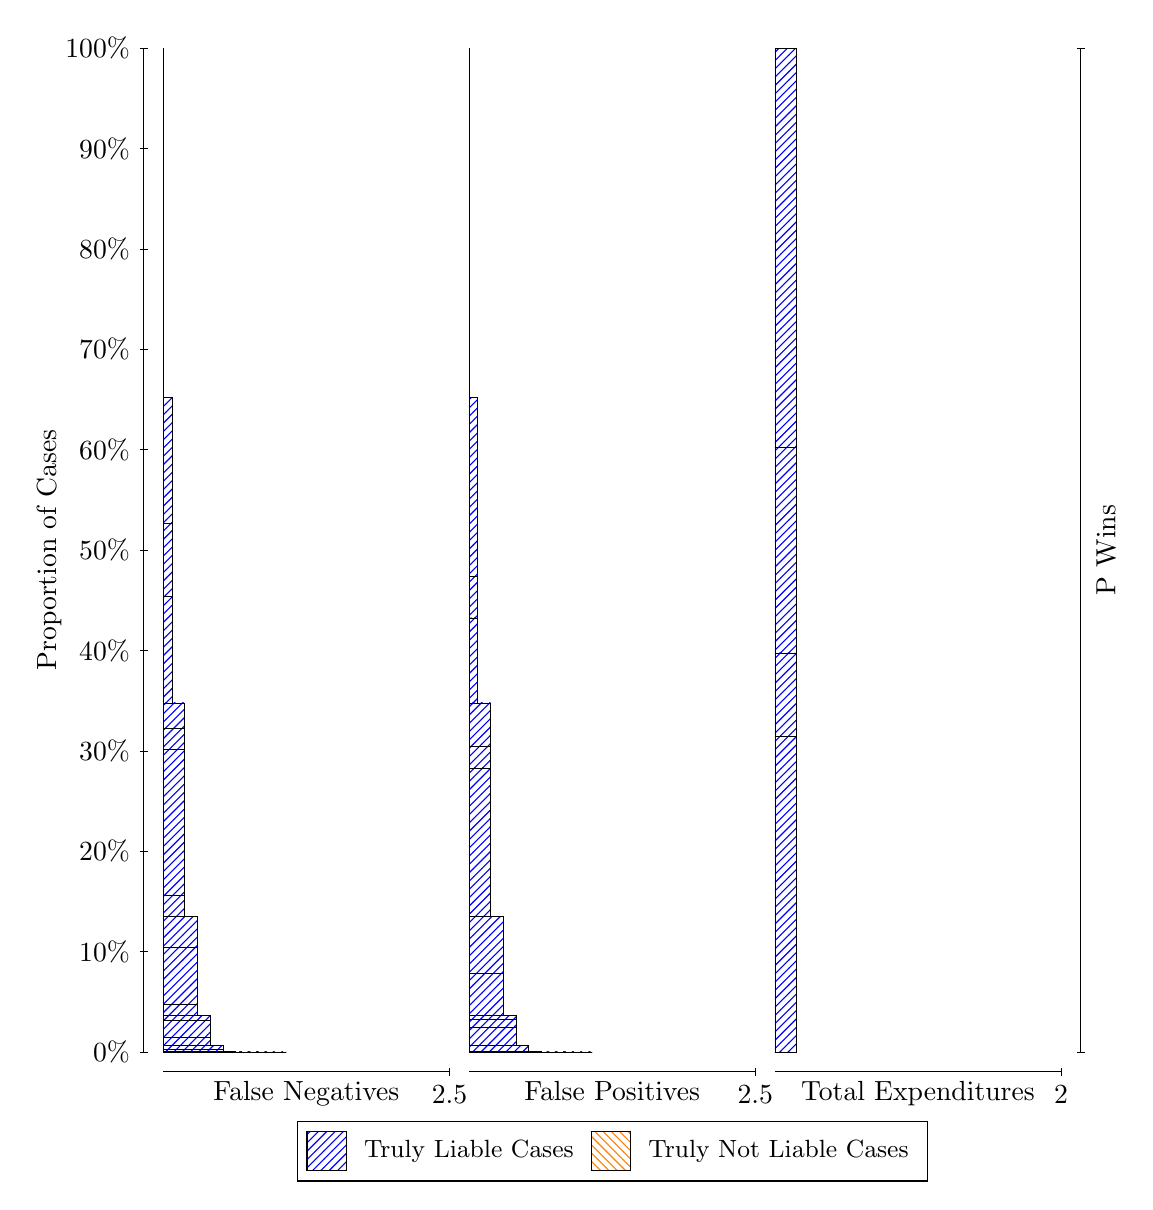
\begin{tikzpicture}
\draw[black, very thin] (1.5,1.75) -- (1.5,14.5);
\node[rotate=90, text=black, anchor=center] at (0.3, 8.125) {Proportion of Cases};
\draw[black, very thin] (1.45,1.75) -- (1.55,1.75);
\node[text=black, anchor=east] at (1.45, 1.75) {0\%};
\draw[black, very thin] (1.45,3.025) -- (1.55,3.025);
\node[text=black, anchor=east] at (1.45, 3.025) {10\%};
\draw[black, very thin] (1.45,4.3) -- (1.55,4.3);
\node[text=black, anchor=east] at (1.45, 4.3) {20\%};
\draw[black, very thin] (1.45,5.575) -- (1.55,5.575);
\node[text=black, anchor=east] at (1.45, 5.575) {30\%};
\draw[black, very thin] (1.45,6.85) -- (1.55,6.85);
\node[text=black, anchor=east] at (1.45, 6.85) {40\%};
\draw[black, very thin] (1.45,8.125) -- (1.55,8.125);
\node[text=black, anchor=east] at (1.45, 8.125) {50\%};
\draw[black, very thin] (1.45,9.4) -- (1.55,9.4);
\node[text=black, anchor=east] at (1.45, 9.4) {60\%};
\draw[black, very thin] (1.45,10.675) -- (1.55,10.675);
\node[text=black, anchor=east] at (1.45, 10.675) {70\%};
\draw[black, very thin] (1.45,11.95) -- (1.55,11.95);
\node[text=black, anchor=east] at (1.45, 11.95) {80\%};
\draw[black, very thin] (1.45,13.225) -- (1.55,13.225);
\node[text=black, anchor=east] at (1.45, 13.225) {90\%};
\draw[black, very thin] (1.45,14.5) -- (1.55,14.5);
\node[text=black, anchor=east] at (1.45, 14.5) {100\%};

\draw[black, very thin] (13.4,1.75) -- (13.4,14.5);
\draw[black, very thin] (13.35,1.75) -- (13.45,1.75);
\node[anchor=west] at (13.35, 1.75) {};
\draw[black, very thin] (13.35,14.5) -- (13.45,14.5);
\node[anchor=west] at (13.35, 14.5) {};

\draw[black, very thin, pattern color=blue, pattern=north east lines] (1.75,1.75) rectangle (3.3123,1.75);
\draw[black, very thin, pattern color=blue, pattern=north east lines] (1.75,1.75) rectangle (3.1509,1.75);
\draw[black, very thin, pattern color=blue, pattern=north east lines] (1.75,1.75) rectangle (3.1509,1.75);
\draw[black, very thin, pattern color=blue, pattern=north east lines] (1.75,1.75) rectangle (2.9894,1.75);
\draw[black, very thin, pattern color=blue, pattern=north east lines] (1.75,1.75) rectangle (2.9894,1.75);
\draw[black, very thin, pattern color=blue, pattern=north east lines] (1.75,1.75) rectangle (2.8279,1.7506);
\draw[black, very thin, pattern color=blue, pattern=north east lines] (1.75,1.7506) rectangle (2.8279,1.7507);
\draw[black, very thin, pattern color=blue, pattern=north east lines] (1.75,1.7507) rectangle (2.6664,1.7599);
\draw[black, very thin, pattern color=blue, pattern=north east lines] (1.75,1.7599) rectangle (2.5049,1.782);
\draw[black, very thin, pattern color=blue, pattern=north east lines] (1.75,1.782) rectangle (2.5049,1.8337);
\draw[black, very thin, pattern color=blue, pattern=north east lines] (1.75,1.8337) rectangle (2.3434,1.933);
\draw[black, very thin, pattern color=blue, pattern=north east lines] (1.75,1.933) rectangle (2.3434,2.1561);
\draw[black, very thin, pattern color=blue, pattern=north east lines] (1.75,2.1561) rectangle (2.3434,2.2136);
\draw[black, very thin, pattern color=blue, pattern=north east lines] (1.75,2.2136) rectangle (2.182,2.3552);
\draw[black, very thin, pattern color=blue, pattern=north east lines] (1.75,2.3552) rectangle (2.182,3.0792);
\draw[black, very thin, pattern color=blue, pattern=north east lines] (1.75,3.0792) rectangle (2.182,3.4713);
\draw[black, very thin, pattern color=blue, pattern=north east lines] (1.75,3.4713) rectangle (2.0205,3.7405);
\draw[black, very thin, pattern color=blue, pattern=north east lines] (1.75,3.7405) rectangle (2.0205,5.5912);
\draw[black, very thin, pattern color=blue, pattern=north east lines] (1.75,5.5912) rectangle (2.0205,5.8626);
\draw[black, very thin, pattern color=blue, pattern=north east lines] (1.75,5.8626) rectangle (2.0205,6.182);
\draw[black, very thin, pattern color=blue, pattern=north east lines] (1.75,6.182) rectangle (1.859,7.5347);
\draw[black, very thin, pattern color=blue, pattern=north east lines] (1.75,7.5347) rectangle (1.859,8.4584);
\draw[black, very thin, pattern color=blue, pattern=north east lines] (1.75,8.4584) rectangle (1.859,10.068);
\draw[black, very thin, pattern color=orange, pattern=north west lines] (1.75,10.068) rectangle (1.75,10.068);
\draw[black, very thin, pattern color=blue, pattern=north east lines] (1.75,10.068) rectangle (1.75,14.5);
\draw[black, very thin, pattern color=orange, pattern=north west lines] (5.6333,1.75) rectangle (7.1957,1.75);
\draw[black, very thin, pattern color=blue, pattern=north east lines] (5.6333,1.75) rectangle (7.1957,1.75);
\draw[black, very thin, pattern color=orange, pattern=north west lines] (5.6333,1.75) rectangle (7.0342,1.75);
\draw[black, very thin, pattern color=blue, pattern=north east lines] (5.6333,1.75) rectangle (7.0342,1.75);
\draw[black, very thin, pattern color=orange, pattern=north west lines] (5.6333,1.75) rectangle (6.8727,1.75);
\draw[black, very thin, pattern color=blue, pattern=north east lines] (5.6333,1.75) rectangle (6.8727,1.75);
\draw[black, very thin, pattern color=blue, pattern=north east lines] (5.6333,1.75) rectangle (6.8727,1.75);
\draw[black, very thin, pattern color=blue, pattern=north east lines] (5.6333,1.75) rectangle (6.7112,1.7504);
\draw[black, very thin, pattern color=orange, pattern=north west lines] (5.6333,1.7504) rectangle (6.7112,1.7504);
\draw[black, very thin, pattern color=blue, pattern=north east lines] (5.6333,1.7504) rectangle (6.7112,1.7507);
\draw[black, very thin, pattern color=orange, pattern=north west lines] (5.6333,1.7507) rectangle (6.5497,1.7507);
\draw[black, very thin, pattern color=blue, pattern=north east lines] (5.6333,1.7507) rectangle (6.5497,1.7599);
\draw[black, very thin, pattern color=orange, pattern=north west lines] (5.6333,1.7599) rectangle (6.3883,1.7599);
\draw[black, very thin, pattern color=blue, pattern=north east lines] (5.6333,1.7599) rectangle (6.3883,1.8337);
\draw[black, very thin, pattern color=orange, pattern=north west lines] (5.6333,1.8337) rectangle (6.2268,1.8337);
\draw[black, very thin, pattern color=blue, pattern=north east lines] (5.6333,1.8337) rectangle (6.2268,2.0587);
\draw[black, very thin, pattern color=blue, pattern=north east lines] (5.6333,2.0587) rectangle (6.2268,2.1651);
\draw[black, very thin, pattern color=blue, pattern=north east lines] (5.6333,2.1651) rectangle (6.2268,2.2136);
\draw[black, very thin, pattern color=orange, pattern=north west lines] (5.6333,2.2136) rectangle (6.0653,2.2136);
\draw[black, very thin, pattern color=blue, pattern=north east lines] (5.6333,2.2136) rectangle (6.0653,2.7486);
\draw[black, very thin, pattern color=blue, pattern=north east lines] (5.6333,2.7486) rectangle (6.0653,3.4713);
\draw[black, very thin, pattern color=orange, pattern=north west lines] (5.6333,3.4713) rectangle (5.9038,3.4713);
\draw[black, very thin, pattern color=blue, pattern=north east lines] (5.6333,3.4713) rectangle (5.9038,5.3592);
\draw[black, very thin, pattern color=blue, pattern=north east lines] (5.6333,5.3592) rectangle (5.9038,5.6306);
\draw[black, very thin, pattern color=blue, pattern=north east lines] (5.6333,5.6306) rectangle (5.9038,6.182);
\draw[black, very thin, pattern color=blue, pattern=north east lines] (5.6333,6.182) rectangle (5.7423,7.2636);
\draw[black, very thin, pattern color=orange, pattern=north west lines] (5.6333,7.2636) rectangle (5.7423,7.2636);
\draw[black, very thin, pattern color=blue, pattern=north east lines] (5.6333,7.2636) rectangle (5.7423,7.7916);
\draw[black, very thin, pattern color=blue, pattern=north east lines] (5.6333,7.7916) rectangle (5.7423,10.068);
\draw[black, very thin, pattern color=blue, pattern=north east lines] (5.6333,10.068) rectangle (5.6333,14.5);
\draw[black, very thin, pattern color=orange, pattern=north west lines] (9.5167,1.75) rectangle (9.7892,1.75);
\draw[black, very thin, pattern color=blue, pattern=north east lines] (9.5167,1.75) rectangle (9.7892,5.7617);
\draw[black, very thin, pattern color=orange, pattern=north west lines] (9.5167,5.7617) rectangle (9.7892,5.7617);
\draw[black, very thin, pattern color=blue, pattern=north east lines] (9.5167,5.7617) rectangle (9.7892,6.819);
\draw[black, very thin, pattern color=orange, pattern=north west lines] (9.5167,6.819) rectangle (9.7892,6.819);
\draw[black, very thin, pattern color=blue, pattern=north east lines] (9.5167,6.819) rectangle (9.7892,9.431);
\draw[black, very thin, pattern color=orange, pattern=north west lines] (9.5167,9.431) rectangle (9.7892,9.431);
\draw[black, very thin, pattern color=blue, pattern=north east lines] (9.5167,9.431) rectangle (9.7892,14.5);
\draw[black, very thin] (1.75,1.5) -- (5.3833,1.5);
\node[text=black, anchor=north] at (3.5667, 1.5) {False Negatives};
\draw[black, very thin] (5.3833,1.45) -- (5.3833,1.55);
\node[text=black, anchor=north] at (5.3833, 1.45) {2.5};

\draw[black, very thin] (5.6333,1.5) -- (9.2667,1.5);
\node[text=black, anchor=north] at (7.45, 1.5) {False Positives};
\draw[black, very thin] (9.2667,1.45) -- (9.2667,1.55);
\node[text=black, anchor=north] at (9.2667, 1.45) {2.5};

\draw[black, very thin] (9.5167,1.5) -- (13.15,1.5);
\node[text=black, anchor=north] at (11.333, 1.5) {Total Expenditures};
\draw[black, very thin] (13.15,1.45) -- (13.15,1.55);
\node[text=black, anchor=north] at (13.15, 1.45) {2};

\node[text=black, centered, rotate=90] at (13.72, 8.125) {P Wins};

\draw (7.449999999999999,1.5) node[draw=none] (baseCoordinate) {};
\begin{scope}[align=center]
        \matrix[scale=0.5, draw=black, below=0.5cm of baseCoordinate, nodes={draw}, column sep=0.1cm]{
            \node[rectangle, draw, minimum width=0.5cm, minimum height=0.5cm, pattern color=blue, pattern=north east lines] {}; &
            \node[draw=none, font=\small, text=black] (B) {Truly Liable Cases}; &
            \node[rectangle, draw, minimum width=0.5cm, minimum height=0.5cm, pattern color=orange, pattern=north west lines] {}; &
            \node[draw=none, font=\small, text=black] (B) {Truly Not Liable Cases}; \\
            };
\end{scope}

\end{tikzpicture}
\end{document}